% File: SliderCrank.tex
% Author: Adam Leeper
%------------------------------------------------------------------------------
%\\[0.45pc]
\providecommand{\isolatedBuild}[1]{#1}% Fallback definition to build normally.
\isolatedBuild{
  \documentclass[11pt,letterpaper]{book}
  %\documentclass[11pt,letterpaper]{book}

% aleeper: I think these are needed for Paul's macros?
\usepackage{epsfig}
\usepackage{epstopdf}

%\makeatletter
%\typeout{The import path is \import@path}
%\makeatother

\usepackage{import}

\subimport{./}{packagesMitiguy.sty}
\subimport{./}{macrosMitiguy.tex}
\subimport{./}{PageStylesMitiguy.tex}
\subimport{./}{macrosLeeper.tex}
   % Found via TEXINPUTS environment variable.
  \isolatedBuildHeader{Slider-Crank}
                      {Slider-Crank}
}
%%%
%%%
%%%
\section{Example: Kinematic Analysis for a Slider-Crank Mechanism}
The following two problems are typical EIT-style slider-crank problems. These problems are sometimes categorized as ``relative motion analysis" and/or "instant-center" methods in traditional textbooks. The purpose of this handout is to demonstrate how to solve this variety of planar kinematics problems without resorting to graphical instant-center methods. The solutions to the two problems could probably be combined and generalized to a set of formulas based on the lengths of the links and configuration angles, but that would defeat the purpose of knowing how to do general kinematics!
%
%\\[0.25pc]
%\begin{enumerate}
% ----------------------------------
%\item
\subsection{Relating Velocity and Angular Velocity}
The figure below shows a slider-crank mechanism. If member AB has a constant angular velocity of 3 radians/sec clockwise, the velocity of slider C at the instant shown is:

\begin{minipage}{0.4\linewidth}
  \begin{itemize}
    \item[a.] 12 in/sec
    \item[b.] 9 in/sec
    \item[c.] 16 in/sec
    \item[d.] 15 in/sec
    \item[e.] zero (it is momentarily at rest)
  \end{itemize}
\end{minipage}
\hfill
\begin{minipage}{0.4\linewidth}
\centering
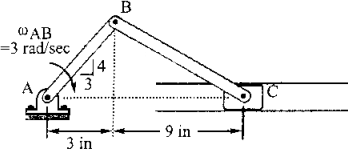
\includegraphics[width=1\linewidth]{slider_crank_1.png}
\end{minipage}
\\[1.0pc]
\textbf{Solution:}
The traditional approach to this problem involves sketching on the picture to graphically find a point that is the instant center of rotation for member BC. However, we can solve it in a more methodical way by considering the velocity equation for two points fixed on a rigid body.
%
\\[1.0pc]
\begin{minipage}{0.4\linewidth}
Let's re-label the drawing using our notation style. Link \basis{A} is connected to \basis{N} by a hinge at $A_o$ and to link \basis{B} by a hinge at $A_B$. Link \basis{C} is modeled as a particle, and is connected to \basis{B} by a hinge. As suggested by the picture, \basis{C} is constrained to slide in the slot horizontally.
\end{minipage}
\hfill
\begin{minipage}{0.4\linewidth}
\centering
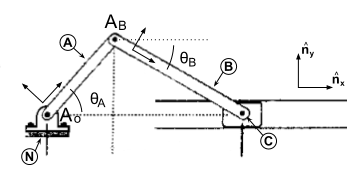
\includegraphics[width=1\linewidth]{slider_crank_1_labeled.png}
\end{minipage}
%
\\[1.0pc]
For convenience, we define our usual \dextral, orthogonal unit vectors fixed in \basis{N} with \uvecx{n} horizontally right and \uvecy{n} vertically upward. Let \basis{A} have similar unit vectors with $\uvecz{a} = \uvecz{n}$ and \uvecx{a} pointing from $A_o$ to $A_B$, and likewise \basis{B} has $\uvecz{b} = \uvecz{n}$ and \uvecx{b} pointing from $A_B$ to $C$.
Then we can write $\angvel{A}{N} = - \omega_A ~\uvecz{n}$
and $\angvel{B}{N} = - \omega_B ~\uvecz{n}$.
%
\\[1.0pc]
Our desired unknown is the measure of C's velocity in the \uvecx{n} direction. To get there, we need to know something about the motion of link \basis{B}, which means we need to know the velocity of $A_B$. Fortunately, since we know the motion of link \basis{A} we can directly compute the velocity of point $A_B$ using the equation for two points fixed on a rigid body:
\\[0.0pc]
$$\vel{A_B}{N} \equals[\;] \vel{A_o}{N} + \angvel{A}{N} \Cross \posvec{A_o}{A_B}
 \equals[\;] \zerovec  \plus[\;] (-\omega_A~\uvecz{n}) \Cross (L_A~\uvecx{a})$$
\\[0.0pc]
And similarly we can relate the velocity of point $A_B$ and point $C$.
\\[0.0pc]
\begin{center}
\begin{tabular}{r@{$\equals[\;]$}r@{$\plus[\;]$}r}
$\vel{C}{N}$ & $\vel{A_B}{N}$ & $\angvel{B}{N} \Cross \posvec{A_B}{C}$
\\[0.45pc]
$v_x~\uvecx{n} + v_y~\uvecy{n}$ & $(-\omega_A~\uvecz{n}) \Cross (L_A~\uvecx{a})$ & $(-\omega_B~\uvecz{n}) \Cross (L_B~\uvecx{b})$
\\[0.45pc]
$v_x~\uvecx{n} + v_y~\uvecy{n}$ & $(-\omega_A~L_A)~\uvecy{a}$ & $(-\omega_B~L_B)~\uvecy{b}$
\end{tabular}
\end{center}
%
%\clearpage
In the above equation there are 3 unknowns ($v_y$, $v_x$, $\omega_B$). We can get 2 scalar equations by dotting with \uvecy{n} and \uvecx{n}, and a third equation by considering the slot constraint, arguing that it enforces $v_y = 0$.
\\[0.0pc]
$$v_y = 0$$
$$v_y \equals[\;] (-\omega_A~L_A)~\uvecy{a}\cdot\uvecy{n} + (-\omega_B~L_B)~\uvecy{b}\cdot\uvecy{n}$$
$$v_x \equals[\;] (-\omega_A~L_A)~\uvecy{a}\cdot\uvecx{n} + (-\omega_B~L_B)~\uvecy{b}\cdot\uvecx{n}$$
%
\\[0.0pc]
The lengths are calculated from the picture:
\\[0.45pc]
\begin{minipage}{0.5\linewidth}
$$L_A = \sqrt{3^2 + 4^2} = 5$$
\end{minipage}
\hfill
\begin{minipage}{0.5\linewidth}
$$L_B = \sqrt{4^2 + 9^2} = 9.85$$
\end{minipage}
%
\\[1.0pc]
Finally, the simple rotation matrices \dircos{N}{A} and \dircos{N}{B} take the form:
\\[0.45pc]
\begin{minipage}{0.5\linewidth}
%$$\angle(\uvecx{a}, \uvecx{n}) = \mathrm{acos}(\frac{3}{5}) = 53.13^\circ$$
\centering
%\simpleRotationZ{n}{a}{53.13^\circ}
\simpleRotationZ{n}{a}{\theta_A}
\end{minipage}
\hfill
\begin{minipage}{0.5\linewidth}
%$$\angle(\uvecx{b}, \uvecx{n}) = \mathrm{atan}(\frac{4}{9}) = 23.96^\circ$$
\centering
%\simpleRotationZ{b}{n}{23.96^\circ}
\simpleRotationZ{b}{n}{\theta_B}
\end{minipage}
%
\\[0.45pc]
which can be filled in either by using trig to compute
$\theta_A = 53.13^\circ$ and $\theta_B =  23.96^\circ$,
or by using ``\textit{soh cah toa}'' to replace the trig functions by the appropriate ratios:
\\[0.45pc]
\begin{minipage}{0.5\linewidth}
\centering
\ensuremath{
   \begin{array}{c|ccc}
      \dircos{n}{a}  &  \uvec{a}{x}  &  \uvec{a}{y}  & \uvec{a}{z} \\[0.0pc]\hline
         \uvec{n}{x}  &  3/5     &  -4/5    & 0    \\[0.0pc]
         \uvec{n}{y}  &  4/5     &   3/5    & 0    \\[0.0pc]
         \uvec{n}{z}  &  0     & 0      & 1
   \end{array} }
\end{minipage}
\hfill
\begin{minipage}{0.5\linewidth}
\centering
\ensuremath{
   \begin{array}{c|ccc}
      \dircos{b}{n}  &  \uvec{n}{x}  &  \uvec{n}{y}  & \uvec{n}{z} \\[0.0pc]\hline
         \uvec{b}{x}  & 9/9.85      &  -4/9.85     & 0    \\[0.0pc]
         \uvec{b}{y}  & 4/9.85      &   9/9.85   & 0    \\[0.0pc]
         \uvec{b}{z}  &  0     & 0      & 1
   \end{array} }
\end{minipage}

So our system of equations reduces to:

$$0 \equals[\;] (-\omega_A~L_A)~\cos(\theta_A) + (-\omega_B~L_B)~(\cos(\theta_B))$$
$$v_x \equals[\;] (-\omega_A~L_A)~(-\sin(\theta_A)) + (-\omega_B~L_B)~(\sin(\theta_B))$$

which is solved as:

$$w_B \equals[\;] (-\omega_A~\frac{L_A}{L_B})~(\frac{3}{5})~(\frac{9.85}{9})
= -3~\mathrm{\frac{rad}{s}}*\frac{5~\mathrm{in}}{9.85~\mathrm{in}}*\frac{3}{5}*\frac{9.85}{9}
= -1~\mathrm{\frac{rad}{s}}$$

$$v_x \equals[\;]
 (-3~\mathrm{\frac{rad}{s}})~(5~\mathrm{in})~(-\frac{4}{5})
+ (1~\mathrm{\frac{rad}{s}})~(9.85~\mathrm{in})~(\frac{4}{9.85})
= 16 \mathrm{\frac{in}{s}}$$
%
\\[1.0pc]
It seems our result matches choice (c) in the question, which is indeed the correct answer.
\\[1.0pc]
It is worth noting that this analysis is quite general; similar slider-crank problems can be solved by computing the lengths and rotation tables given whatever new pictorial geometry is presented.

\clearpage
% ----------------------------------

\subsection{Relating Acceleration and Angular Acceleration}
Below is shown a mechanism consisting of a rotating disk AB, a link BC, and a slider at C.
The wheel AB has a constant angular velocity of 6 radians/sec.
At the instant shown, the link BC is translating (its angular velocity is zero).
The angular acceleration of link BC is:
\\[-0.45pc]
\begin{minipage}[t]{0.4\linewidth}
  \vspace*{0pt}
  \begin{itemize}
    \item[a.] 0
    \item[b.] 15 rad/sec$^2$ CCW
    \item[c.] 9 rad/sec$^2$ CW
    \item[d.] 6 rad/sec$^2$ CCW
    \item[e.] 13 rad/sec$^2$ CW
  \end{itemize}
\end{minipage}
\hfill
\begin{minipage}[t]{0.4\linewidth}
  \vspace*{0pt}
  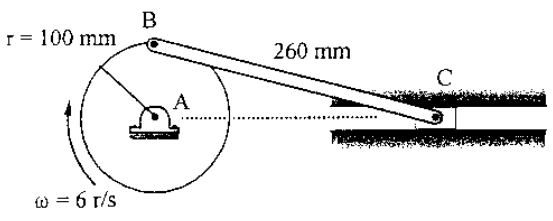
\includegraphics[width=1.0\linewidth]{slider_crank_2.png}
\end{minipage}
\\[0.45pc]
%
\textbf{Solution:}
%
\\[0.45pc]
\begin{minipage}[t]{0.5\linewidth}
  We will once again use the two-points-fixed equations to analyze the
  kinematics, although this time we will need to use the acceleration
  equation as well as the velocity equation.
  \\[0.45pc]
  Let's re-label the drawing using our notation style. The configuration
  of the mechanism has been changed slightly to better show the angles
  and basis vectors we've assigned. Not shown on the drawing are $r_A$,
  the radius of the wheel, and $L_B$, the length of link \basis{B}.
\end{minipage}
\hfill
\begin{minipage}[t]{0.4\linewidth}
  \vspace*{0pt}
  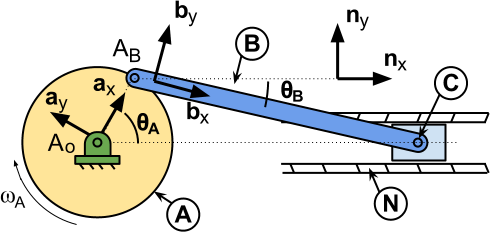
\includegraphics[width=1.0\linewidth]{slider_crank_2_labeled.png}
\end{minipage}
%
\\[1.0pc]
For convenience, we define our usual \dextral, orthogonal unit vectors fixed in \basis{N} with \uvecx{n} horizontally right and \uvecy{n} vertically upward. Let \basis{A} have similar unit vectors with $\uvecz{a} = \uvecz{n}$ and \uvecx{a} pointing from $A_o$ to $A_B$, and likewise \basis{B} has $\uvecz{b} = \uvecz{n}$ and \uvecx{b} pointing from $A_B$ to $C$.
%Then we can write $\angvel{A}{N} = - \omega_A ~\uvecz{n}$
%and $\angvel{B}{N} = - \omega_B ~\uvecz{n}$.
%
\\[0.45pc]
Going with the clockwise convention suggested in the picture, we express the angular velocities and angular accelerations as:
\\[0.0pc]
\begin{minipage}{0.4\linewidth}
\centering
$\angvel{A}{N} = -\omega_A~\uvecz{a}$
\\[0.25pc] $\alf{A}{N} = -\omegadot_A~\uvecz{a}$
\end{minipage}
\begin{minipage}{0.4\linewidth}
\centering
$\angvel{B}{N} = -\omega_B~\uvecz{b}$
\\[0.25pc] $\alf{B}{N} = -\omegadot_B~\uvecz{b}$
\end{minipage}
%
\\[0.45pc]
As before, the simple rotation matrices \dircos{N}{A} and \dircos{N}{B} take the form
\\[0.45pc]
\begin{minipage}{0.5\linewidth}
%$$\angle(\uvecx{a}, \uvecx{n}) = \mathrm{acos}(\frac{3}{5}) = 53.13^\circ$$
\centering
%\simpleRotationZ{n}{a}{53.13^\circ}
\simpleRotationZ{n}{a}{\theta_A}
\end{minipage}
\hfill
\begin{minipage}{0.5\linewidth}
%$$\angle(\uvecx{b}, \uvecx{n}) = \mathrm{atan}(\frac{4}{9}) = 23.96^\circ$$
\centering
%\simpleRotationZ{b}{n}{23.96^\circ}
\simpleRotationZ{b}{n}{\theta_B}
\end{minipage}
%
\\[0.45pc]
where $\theta_A = 90^\circ$ and $\theta_B = 22.62^\circ$ at the instant considered in the problem (found using trig).
%
\\[0.45pc]
For link \basis{B}, we can relate its angular acceleration to the acceleration of the end-points by:
\begin{equation}\label{eqn:slider_crank_accel_c_n}
\accel{C}{N} \equals[\;] \accel{A_B}{N} \plus[\;] \alf{B}{N} \Cross \posvec{A_B}{C} \plus[\;] \angvel{B}{N} \Cross (\angvel{B}{N} \Cross \posvec{A_B}{C})
\end{equation}
which suggests that we need to find the acceleration of $A_B$ and of $C$, and the angular velocity of \basis{B}.
%
\\[0.45pc]
We can get the acceleration of $A_B$ by:
\\[0.0pc]
$$ \accel{A_B}{N} \equals[\;] \accel{A_o}{N} \plus[\;] \alf{A}{N} \Cross \posvec{A_o}{A_B} \plus[\;] \angvel{A}{N} \Cross (\angvel{A}{N} \Cross \posvec{A_o}{A_B})$$
$$ \accel{A_B}{N} \equals[\;] \zerovec \plus[\;] (-\omegadot_A~\uvecz{a}) \Cross (r_A~\uvecx{a}) \plus[\;] -\omega_A~\uvecz{a} \Cross (-\omega_A~\uvecz{a} \Cross r_A~\uvecx{a})$$
\begin{equation}\label{eqn:slider_crank_accel_ab_n}
\accel{A_B}{N} \equals[\;] -r_A \omegadot_A~\uvecy{a}
\minus[\;] r_A \omega_A^2~\uvecx{a}
\end{equation}
\\[0.0pc]
Plugging equation (\ref{eqn:slider_crank_accel_ab_n}) into
(\ref{eqn:slider_crank_accel_c_n}), and assuming that \accel{C}{N}
is of the form $\accel{C}{N} = a_x~\uvecx{n} \plus[\;] 0~\uvecy{n}$
(by physical reasoning, the slot constraint enforces that there is only a
horizontal component) we get:
$$ a_x~\uvecx{n} \plus[\;] 0~\uvecy{n} \equals[\;] -r_A \omegadot_A~\uvecy{a}
   \minus[\;] r_A \omega_A^2~\uvecx{a} \plus[\;] (-\omegadot_B~\uvecz{b})
   \Cross L_B~\uvecx{b} \plus[\;] (-\omega_B~\uvecz{b}) \Cross (-\omega_B~\uvecz{b} \Cross L_B~\uvecx{b})
$$
\begin{equation}
a_x~\uvecx{n} \plus[\;] 0~\uvecy{n} \equals[\;] -r_A \omegadot_A~\uvecy{a}
\minus[\;] r_A \omega_A^2~\uvecx{a} \minus[\;] \omegadot_B L_B ~\uvecy{b}
\minus[\;] \omega_B^2 L_B~\uvecx{b}
\end{equation}

Note that, so far, we haven't assumed a constant rate of rotation of \basis{A}.
Now we can simplify our expression by plugging in $\omegadot_A = 0$ and $\omega_B = 0$ as stated in the problem:
\\[0.0pc]
\begin{equation}
\label{eqn:slider_crank_p2_final_expression}
a_x~\uvecx{n} \equals[\;]
\minus[\;] r_A \omega_A^2~\uvecx{a}
\minus[\;] \omegadot_B L_B ~\uvecy{b}
\end{equation}

We are left with two unknowns.
Dotting equation \ref{eqn:slider_crank_p2_final_expression} with any two
independent unit vectors will give us two independent scalar equations;
let's pick \uvecx{n} and \uvecy{n} for simple look-up in the rotation tables:
%
\\[0.45pc]
\begin{minipage}{0.4\linewidth}
\centering
dot w/ \uvecx{n}:
\\[0.0pc] dot w/ \uvecy{n}:
\end{minipage}
\begin{minipage}{0.4\linewidth}
$a_x \equals[\;]
\minus[\;] r_A \omega_A^2 \cos(\theta_A) \minus[\;] \omegadot_B L_B \sin(\theta_B)$
\\[0.0pc]
$0 \equals[\;]
\minus[\;] r_A \omega_A^2 \sin(\theta_A) \minus[\;] \omegadot_B L_B \cos(\theta_B)$
\end{minipage}
%
\\[0.45pc]
Plugging in $\theta_A = 90^\circ$, $\theta_B = 22.62^\circ$, $\omega_A = 6$ rad/s, $r_A = 100$ mm, and $L_B = 260$ mm, we find:

$$\omegadot_B \equals[\;] -15~\mathrm{rad/s^2}$$
$$a_x \equals[\;] 1500~\mathrm{mm/s^2} \equals[\;] 1.5~\mathrm{m/s^2}$$

And finally we find that answer (b) is the correct choice:
$$\alf{B}{N} = -\omegadot_B~\uvecz{b} = + 15~\mathrm{rad/s^2}~\uvecz{b} = 15~\mathrm{rad/s^2}~\mathrm{CCW}$$

\textbf{Addendum:}
\\[0.0pc]
The problem tells us $\omega_B = 0$ at the instant shown, but let's prove it using the two-points-fixed velocity equation:
\\[0.0pc]
$$\vel{A_B}{N} \equals[\;] \vel{A_o}{N} + \angvel{A}{N} \Cross \posvec{A_o}{A_B}
 \equals[\;] \zerovec  + (-\omega_A~\uvecz{n}) \Cross (L_A~\uvecx{a})$$
 which we can plug into:
$$\vel{C}{N} \equals[\;] \vel{A_B}{N} + \angvel{B}{N} \Cross \posvec{A_B}{C}$$
$$v_x~\uvecx{n} + 0~\uvecy{n} \equals[\;] (-\omega_A~\uvecz{n})
  \Cross (L_A~\uvecx{a}) + (-\omega_B~\uvecz{n}) \Cross (L_B~\uvecx{b})$$
\begin{equation}\label{eqn:slider_crank_p2_velocity_relation}
  v_x~\uvecx{n} \equals[\;] (-\omega_A~L_A)~\uvecy{a}
                            \plus[\;] (-\omega_B~L_B)~\uvecy{b}
\end{equation}
%
\\[0.0pc]
Dotting equation (\ref{eqn:slider_crank_p2_velocity_relation}) with any two independent unit vectors lets one solve for the unknowns $v_x$ and $w_B$:
\\[0.45pc]
\begin{minipage}{0.4\linewidth}
\centering
dot w/ \uvecx{n}:
\\[0.0pc] dot w/ \uvecy{n}:
\end{minipage}
\begin{minipage}{0.4\linewidth}
$v_x \equals[\;]
 \omega_A L_A \sin(\theta_A) \minus[\;] \omega_B L_B \sin(\theta_B)$
\\[0.0pc]
$0 \equals[\;]
 \omega_A L_A \cos(\theta_A) \minus[\;] \omega_B L_B \cos(\theta_B)$
 \end{minipage}
%
\\[0.45pc]
The result is $\omega_B = 0$ when $\theta_A = 90^\circ$.

% ----------------------------------
%\end{enumerate}

\isolatedBuildFooter

